\section{Results}
\label{sec:results}

\subsection{Accuracy and dynamical fidelity of the surrogates}
\label{sec:res_fidelity}

Table~\ref{tab:surrogates} summarizes the surrogates. The archived L96-20 surrogates reduce the one-step mean-square error of persistence, $\hat{\mathbf x}_{k+1}=\mathbf x_k$, only by a factor of $2.2$, so that their defects are about two thirds of the change of the state over one step. Training the same architecture on the same data for 150 and 2000 epochs reduces the test error by factors of 13 and 59, and the FNOs reduce the persistence error by a factor of about 680. The L96-2000 surrogates still have a test error about ten times larger than their training error, which indicates that their accuracy is limited by the coverage of the 20-dimensional attractor by a single trajectory of 140 time units.

\begin{table}[t]
\centering
\footnotesize
\caption{Surrogates. One-step test MSE (median and range over five seeds, standardized units), reduction with respect to persistence, leading Lyapunov exponent of the surrogate along the reference trajectory and along its own free rollout (mean over seeds; the reference values are $1.565$ for Lorenz--96 and $0.0494$ for Kuramoto--Sivashinsky), and behavior of free rollouts of $4{,}000$ steps.}
\label{tab:surrogates}
\begin{tabular}{lcccll}
\toprule
 & one-step MSE & $\frac{\text{persistence}}{\text{MSE}}$ & $\lambda_1$, reference path & $\lambda_1$, free run & free rollout\\
\midrule
L96-20   & $1.1\times10^{-3}$ ($0.9$--$1.3$) & 2.2 & $1.48\pm0.11$ & -- & diverges (5/5)\\
L96-150  & $8.8\times10^{-5}$ ($8.2$--$10.5$) & 29 & $1.60\pm0.15$ & $1.68$ & amplitude $\times1.3$--$140$\\
L96-2000 & $1.9\times10^{-5}$ ($1.6$--$2.2$) & 144 & $1.56\pm0.15$ & $1.56$ & amplitude $\times1.005$\\
KS       & $4.1\times10^{-6}$ ($2.6$--$6.8$) & 680 & $0.048\pm0.005$ & $0.038$ & amplitude $\times1.02$\\
\bottomrule
\end{tabular}
\end{table}

Along the reference trajectory, the leading Lyapunov exponents of all surrogates are close to that of the reference map, so that the tangent dynamics that transport the defects are reproduced reasonably well even by the least accurate models. The free rollouts behave very differently. All five L96-20 surrogates leave the attractor and diverge after $1{,}700$ to $3{,}700$ steps (27 to 57 Lyapunov times), and the L96-150 surrogates settle on sets whose amplitude exceeds that of the reference attractor (by a median factor of $1.3$, and by more than one order of magnitude for two seeds). Only the L96-2000 surrogates stay on an attractor with the reference amplitude and reproduce the leading exponent in free run. These differences are already visible within the diagnostic horizons (Fig.~\ref{fig:growth}). The median error of L96-20 reaches the saturation level $E_{\rm sat}=(2\operatorname{tr}\operatorname{Cov}[\mathbf x])^{1/2}$, the expected distance between two independent states of the attractor, at about one Lyapunov time, and it exceeds that level by a factor of eight at five Lyapunov times. Any analysis of the L96-20 surrogates beyond about half a Lyapunov time is therefore affected by this drift. In what follows, ``L96'' denotes the L96-2000 surrogates, and the other two families are used to show how the budget changes with the accuracy of the surrogate.

\begin{figure}[t]
\centering
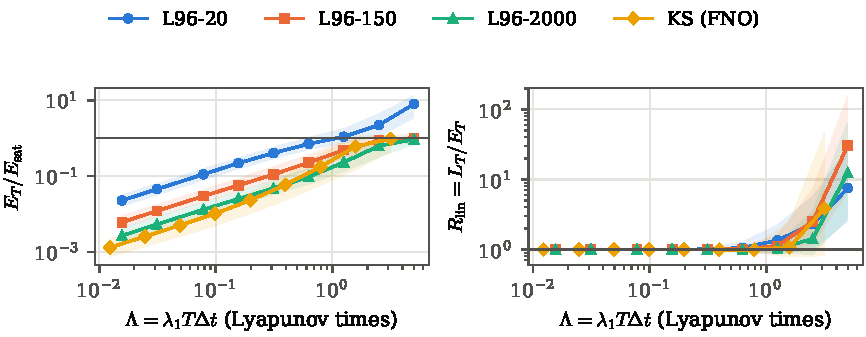
\includegraphics[width=\textwidth]{figures/fig_growth.pdf}
\caption{Error growth. Left: median rollout error relative to the saturation level $E_{\rm sat}$, with 10--90\% bands, as a function of the horizon in Lyapunov times. Right: ratio $R_{\rm lin}$ between the first-order reconstruction and the actual error.}
\label{fig:growth}
\end{figure}

\subsection{Scalar sensitivities}
\label{sec:res_scalar}

Figure~\ref{fig:scalar} shows the within-seed rank correlation between the rollout error and scalar descriptors of the window, as the median over seeds. The worst-case gains $G_{\max}$ and $\|\mathcal L_T\|_2$ and the leading singular value of the one-step Jacobian at the initial state are weak predictors of the error at all horizons. For L96 their correlations lie between $0.09$ and $0.49$, and for KS between $-0.13$ and $0.51$. The total defect magnitude $S_T$ ranks the errors almost perfectly at short horizons and loses most of its value at about one Lyapunov time ($0.49$ for L96 at $\Lambda=1.25$ and $-0.28$ for KS at $\Lambda=0.79$). The norm of the first-order reconstruction keeps a correlation above $0.97$ up to $1.25$ Lyapunov times for L96 and up to $0.79$ Lyapunov times for KS. This is expected, since $\delta^{\rm lin}_T$ is the first-order approximation of $\delta_T$, and it is not an independent explanation of the error. The following sections identify which part of the reconstruction carries the differences between forecasts.

\begin{figure}[t]
\centering
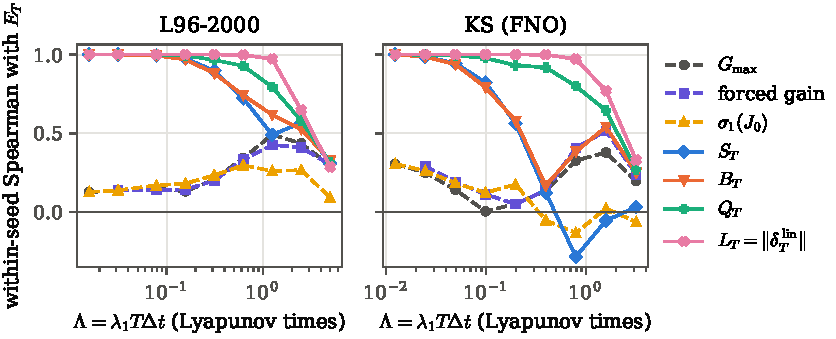
\includegraphics[width=\textwidth]{figures/fig_scalar.pdf}
\caption{Median over seeds of the within-seed Spearman correlation between the rollout error $E_T$ and scalar descriptors of the forecast window. Dashed lines: sensitivity of the learned dynamics only (worst-case initial-value gain, worst-case forced gain and one-step Jacobian). Solid lines: quantities built from the actual defects.}
\label{fig:scalar}
\end{figure}

\subsection{The error budget}
\label{sec:res_budget}

Figure~\ref{fig:budget} shows the five factors of Proposition~\ref{prop:factorization} as geometric means over windows, together with the variance shares of Proposition~\ref{prop:attribution}, and Table~\ref{tab:representative} gives median values at representative horizons. The typical error is built in the same way in both systems. The defect magnitude $S_T$ grows linearly with the horizon and the worst-case tail gain $\bar g_T$ grows approximately exponentially, whereas the efficiency and the cancellation decrease. For L96 at $1.25$ Lyapunov times, the median worst-case estimate $B_T$ exceeds the realized error by a factor of $6.5$, of which a factor of about $3.3$ is removed by the efficiency ($\eta_T=0.31$) and a factor of $1.8$ by the cancellation ($C_T=0.55$). For KS at $0.79$ Lyapunov times, the corresponding values are $4.9$, $\eta_T=0.27$ and $C_T=0.78$, so that the efficiency removes most of the difference.

\begin{figure}[t]
\centering
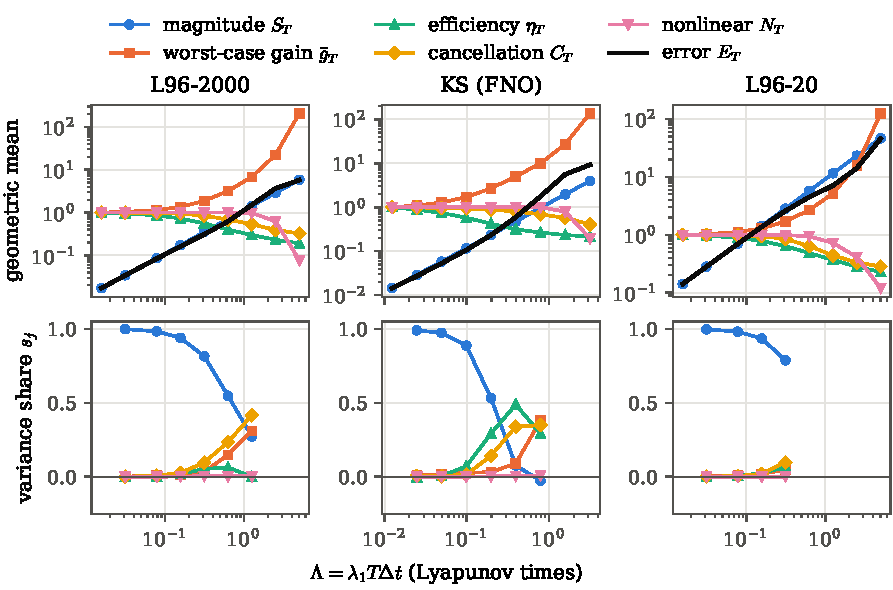
\includegraphics[width=\textwidth]{figures/fig_budget.pdf}
\caption{Error budget. Top: geometric mean over windows of the five factors of Eq.~\eqref{eq:factorization} and of the rollout error. Bottom: variance shares of the log-error (Proposition~\ref{prop:attribution}, within-seed), shown where the median error is below half of the saturation level.}
\label{fig:budget}
\end{figure}

\begin{table}[t]
\centering
\small
\caption{Medians of the budget at representative horizons, and within-seed variance shares of the log-error. $B_T/E_T$ is the ratio between the worst-case first-order estimate and the realized error.}
\label{tab:representative}
\begin{tabular}{lrrrrr}
\toprule
 & L96, $T=40$ & L96, $T=80$ & KS, $T=32$ & KS, $T=64$ & KS, $T=128$\\
\midrule
$\Lambda$ & 0.63 & 1.25 & 0.40 & 0.79 & 1.58\\
$E_T/E_{\rm sat}$ & 0.095 & 0.232 & 0.059 & 0.175 & 0.608\\
$R_{\rm lin}$ & 1.000 & 1.023 & 0.995 & 0.992 & 1.078\\
\midrule
$B_T/E_T$ & 3.6 & 6.5 & 3.6 & 4.9 & 8.1\\
$\bar g_T$ & 3.2 & 6.6 & 4.9 & 9.1 & 23.0\\
$\eta_T$ & 0.40 & 0.31 & 0.32 & 0.27 & 0.24\\
$\eta^\Sigma_T$ & 0.42 & 0.32 & 0.32 & 0.28 & 0.25\\
$\eta^{\rm iso}_T$ & 0.43 & 0.33 & 0.14 & 0.11 & 0.10\\
$\alpha_T$ & 0.96 & 0.94 & 1.03 & 0.97 & 0.96\\
$C_T$ & 0.70 & 0.55 & 0.85 & 0.78 & 0.67\\
$\kappa_T$ & 4.2 & 4.3 & 4.4 & 5.0 & 5.2\\
$\kappa^{\rm iid}_T$ & 1.05 & 1.06 & 1.24 & 1.26 & 1.23\\
$T_{\rm eff}^{1/2}$ & 6.1 & 8.0 & 5.2 & 6.7 & 8.2\\
\midrule
$s_S$ & 0.55 & 0.27 & 0.08 & -0.03 & 0.02\\
$s_{\bar g}$ & 0.15 & 0.31 & 0.09 & 0.38 & 0.61\\
$s_\eta$ & 0.06 & -0.00 & 0.49 & 0.29 & 0.14\\
$s_C$ & 0.24 & 0.41 & 0.34 & 0.35 & 0.39\\
$s_N$ & 0.01 & 0.00 & 0.01 & 0.01 & -0.15\\
\bottomrule
\end{tabular}

\end{table}

The variance shares identify the factors that make some forecasts worse than others. At short horizons, the defect magnitude carries almost all of the variance of the log-error (shares above $0.8$ up to $0.3$ Lyapunov times for L96 and up to $0.1$ Lyapunov times for KS), so that the forecasts that degrade first are those that start in regions of the attractor where the surrogate fits the one-step map less accurately. Geometric factors then replace the magnitude, in a different order in the two systems. For L96, the cancellation and the worst-case gain grow first, and at $1.25$ Lyapunov times their shares ($0.41$ and $0.31$) exceed that of the magnitude ($0.27$, two-level bootstrap interval $[0.20,0.35]$), while the efficiency carries no variance. For KS, the efficiency replaces the magnitude much earlier, with a share of $0.49$ at $0.40$ Lyapunov times, and it is followed by the cancellation and by the worst-case gain, whose share reaches $0.61$ at $1.58$ Lyapunov times. Almost all of the share of the efficiency comes from the orientation ratio $\alpha_T$ ($0.46$, with interval $[0.36,0.65]$, at $0.40$ Lyapunov times), that is, from the variation between windows of the alignment of the defects with the amplified directions. The nonlinear factor carries no variance while the first-order description holds, and its share becomes negative near saturation, where the windows with the largest first-order reconstructions are compressed the most.

The budget changes little with the accuracy of the surrogate. At $0.31$ Lyapunov times, the shares of the magnitude, the cancellation and the worst-case gain differ by at most $0.03$ between the three Lorenz--96 families, and at $0.63$ Lyapunov times they are $0.53$, $0.23$ and $0.13$ for L96-150, against $0.55$, $0.24$ and $0.15$ for L96-2000 (Appendix~\ref{app:tables}). A fiftyfold reduction of the one-step error therefore reduces the error at a given horizon mostly through the magnitude factor, and the dimensionless factors are set mainly by the reference dynamics and by the statistics of the defects.

\subsection{Directional efficiency and the defect covariance}
\label{sec:res_efficiency}

Figure~\ref{fig:efficiency} compares the efficiency of the actual defects with the two null models of Eq.~\eqref{eq:alpha}. For L96, the covariance-matched and isotropic nulls are almost identical, since the defect covariance of the standardized cyclic system is close to isotropic, and the actual efficiency follows both closely. The median orientation ratio is between $0.94$ and $0.99$ up to $1.25$ Lyapunov times. For KS, the isotropic null is much lower than the actual efficiency ($0.11$ against $0.27$ at $0.79$ Lyapunov times), because the defects of the FNO are smooth fields that project mostly on the large scales, which the tail propagators amplify, whereas a random vector of $\R^{64}$ puts most of its energy in strongly damped small scales. Once the spatial structure of the defects is taken into account through $\Sigma$, the actual efficiency is again close to the null, with median orientation ratios between $1.03$ and $1.07$ up to $0.4$ Lyapunov times and of $0.97$ and $0.96$ at $0.79$ and $1.58$ Lyapunov times. For KS, the orientation ratio varies widely between windows (10--90\% range of $[0.56,1.52]$ at $0.79$ Lyapunov times), and this variation carries the share of the efficiency.

\begin{figure}[t]
\centering
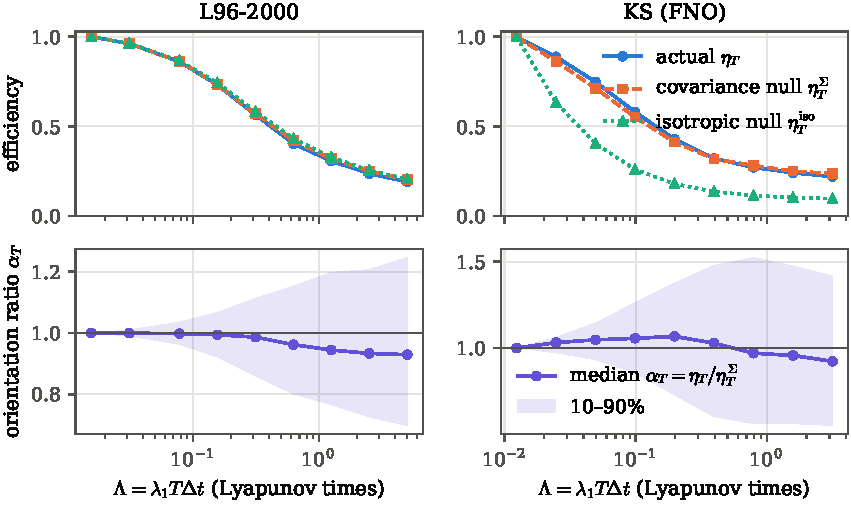
\includegraphics[width=\textwidth]{figures/fig_efficiency.pdf}
\caption{Directional efficiency. Top: median efficiency of the actual defects compared with random defects with the same second moment ($\eta^\Sigma_T$) and with isotropic random defects ($\eta^{\rm iso}_T$), both computed with the mean norm gain of Eq.~\eqref{eq:mean_gain}. Bottom: orientation ratio $\alpha_T=\eta_T/\eta^\Sigma_T$, median and 10--90\% band.}
\label{fig:efficiency}
\end{figure}

The defects of the surrogates are therefore neither attracted to nor repelled by the directions that the dynamics amplify. On average, they realize the fraction of the worst-case gain expected for random draws from their own covariance, within $7\%$ for both systems at all horizons where the first-order description holds. The efficiency decreases with the horizon because, as the singular spectrum of the tail propagators spreads, a vector with a given covariance realizes a decreasing fraction of the leading gain (Proposition~\ref{prop:nulls}). The root-mean-square gains of Proposition~\ref{prop:nulls} would instead have given ratios of $0.89$ at $1.25$ and $0.80$ at five Lyapunov times for L96, close to the Jensen gap $(2/\pi)^{1/2}$, and suggested, incorrectly, that the defects avoid the amplified directions.

The same conclusion holds for the occupation of the singular spectrum (Fig.~\ref{fig:spectrum}). The number of singular directions that carry $90\%$ of the transported energy decreases with the horizon, from $17.6$ at $T=2$ to $3.6$ at five Lyapunov times for L96 (means over defect--tail pairs), and random defects drawn from the defect covariance give $17.5$ and $3.5$. For KS, the actual defects give $6.5$ at $T=2$ and $1.6$ at $3.2$ Lyapunov times, against $7.3$ and $1.6$ for the covariance null, and only the isotropic null departs from them at short horizons ($16.3$ at $T=2$). The concentration of the transported energy in a few leading directions is therefore a property of the propagators and would be observed for any defect.

\begin{figure}[t]
\centering
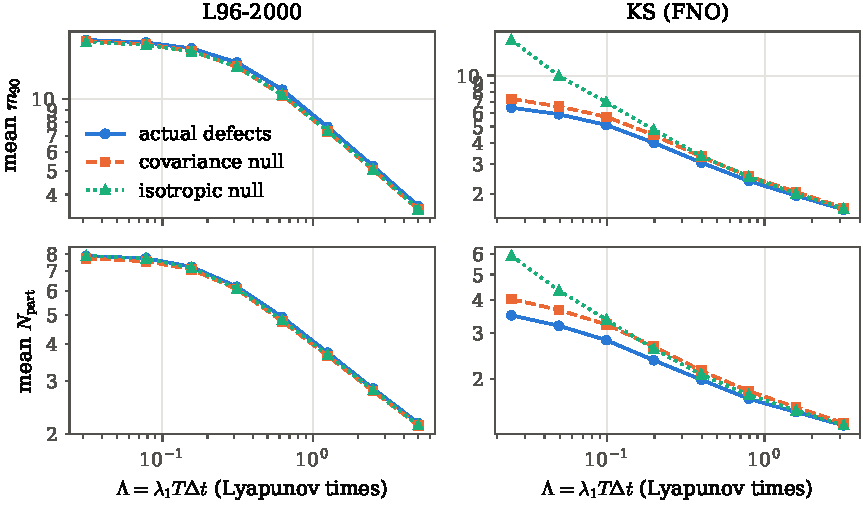
\includegraphics[width=\textwidth]{figures/fig_spectrum.pdf}
\caption{Occupation of the singular spectrum of the tail propagators by the transported defects: number of directions carrying $90\%$ of the energy ($m_{90}$) and participation number, averaged over defect--tail pairs, for the actual defects and for 16 random defects per pair drawn from the covariance-matched and isotropic null models.}
\label{fig:spectrum}
\end{figure}

\subsection{Coherence of the transported defects}
\label{sec:res_coherence}

Figure~\ref{fig:coherence} decomposes the cancellation according to Eq.~\eqref{eq:coherence}. The transported defects are far from incoherent. The coherence factor grows from $\kappa_T=3.8$ at $0.31$ to $4.3$ at $1.25$ Lyapunov times for L96, and from $4.4$ at $0.40$ to $5.2$ at $1.58$ Lyapunov times for KS, against $T_{\rm eff}^{1/2}$ between $4.4$ and $8.2$ for perfectly coherent contributions. The bias of the surrogates explains only a small part of this coherence. Defects drawn independently from a distribution with the same mean and second moment would give $\kappa^{\rm iid}_T$ between $1.04$ and $1.06$ for L96 and about $1.25$ for KS (Eq.~\ref{eq:kappa_iid}), so that the coherence is produced by the temporal correlation of the defects along the trajectory. As the horizon grows, the tail propagators rotate the transported defects into a few leading directions, and the coherence saturates at about four to five while $T_{\rm eff}$ keeps increasing. In the variance attribution, most of the share of the cancellation is carried by $\kappa_T$ (for L96, $0.20$ of $0.24$ at $0.63$ Lyapunov times and $0.32$ of $0.41$ at $1.25$), so that the forecasts with the largest errors are, to a large extent, those whose transported defects add more coherently.

\begin{figure}[t]
\centering
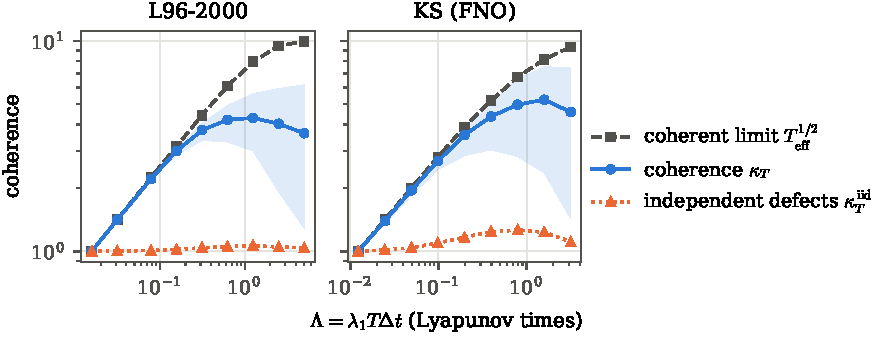
\includegraphics[width=\textwidth]{figures/fig_coherence.pdf}
\caption{Coherence factor $\kappa_T$ of the transported defects (median and 10--90\% band), compared with the coherent limit $T_{\rm eff}^{1/2}$ and with the coherence $\kappa^{\rm iid}_T$ of independent defects with the same mean and second moment (Eq.~\ref{eq:kappa_iid}), which equals one for unbiased defects.}
\label{fig:coherence}
\end{figure}

\subsection{Validity of the first-order reconstruction}
\label{sec:res_validity}

The ratio $R_{\rm lin}$ stays within $2.3\%$ of one up to $1.25$ Lyapunov times for L96, with a median of $1.42$ at $2.5$ Lyapunov times (Fig.~\ref{fig:growth}). For KS, it stays within $1\%$ of one up to $0.79$ Lyapunov times, and its median is $1.08$ at $1.58$ and $3.9$ at $3.2$ Lyapunov times. The departure from the first-order description is controlled by the size of the error relative to the attractor rather than by the horizon (Fig.~\ref{fig:validity}). The median $|\log R_{\rm lin}|$ grows approximately as a power of $E_T/E_{\rm sat}$ and reaches $0.05$ at $E_T/E_{\rm sat}\approx0.20$ for L96, $0.17$ for KS, $0.29$ for L96-150 and $0.54$ for L96-20. The growth is faster for the MLPs (exponents between $2.1$ and $2.5$) than for the FNOs (exponent close to $1.3$). For the accurate surrogates, the first-order reconstruction can therefore be trusted while the rollout error remains below about $15$ to $20\%$ of the saturation level, which corresponds to about one Lyapunov time.

\begin{figure}[t]
\centering
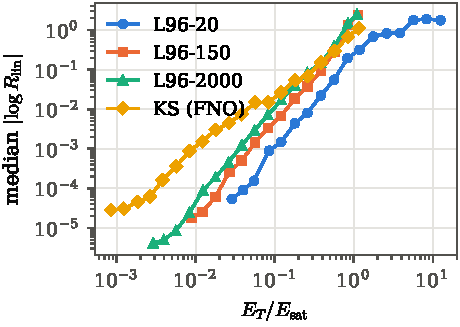
\includegraphics[width=0.6\textwidth]{figures/fig_validity.pdf}
\caption{Median departure from the first-order description, $|\log R_{\rm lin}|$, as a function of the rollout error relative to the saturation level, for windows binned by $E_T/E_{\rm sat}$ and pooled over horizons.}
\label{fig:validity}
\end{figure}

\subsection{Reference-free estimates of the realized error}
\label{sec:res_ensemble}

Since the realized error is determined by the actual defect field and not by its statistics, scores that use only the defect statistics do not rank individual forecasts. For L96, the within-seed rank correlation of $S^{\rm white}_T$ with the error is between $0.08$ and $0.17$ up to $0.31$ Lyapunov times and $0.44$ at $1.25$ Lyapunov times, and the worst-case gain of the model-trajectory propagator behaves in the same way (Fig.~\ref{fig:ensemble}).

The ensemble proxy of Eq.~\eqref{eq:proxy} estimates the defect field itself: on the reference states, its median cosine with the true defect is $0.82$ for the L96-2000 surrogates and $0.84$ for the FNOs, and its median norm is $1.01$ and $1.06$ times the true one, close to the values $0.89$ and $1.12$ expected for independent member errors. This estimate makes the forced recursion usable before the fact (Table~\ref{tab:ensemble} and Fig.~\ref{fig:ensemble}). For L96-2000, the ensemble spread $D_T$ ranks the errors with within-seed correlations between $0.75$ and $0.84$ and flags the 10\% largest errors of each seed with AUROCs between $0.92$ and $0.95$ up to $1.25$ Lyapunov times, and its median ratio to the realized error is between $1.00$ and $1.01$, so that the spread of four other surrogates gives a calibrated estimate of the error of each member. The propagated proxy $\hat L_T$ gives almost the same ranking at the cost of one Jacobian--vector product per step, whereas the proxy magnitude $\hat S_T$ and the one-step proxy fall to $0.50$ and $0.38$ at $1.25$ Lyapunov times. For KS, $D_T$ and $\hat L_T$ keep correlations between $0.67$ and $0.77$ between $0.4$ and $0.8$ Lyapunov times, with AUROCs between $0.92$ and $0.97$, while the magnitude scores become uninformative ($\hat S_T$ has a correlation of $-0.23$ at $0.79$ Lyapunov times). The spread overestimates the KS errors by $7$ to $19\%$ up to $0.79$ Lyapunov times, as expected for nearly independent member errors.

\begin{table}[t]
\centering
\small
\caption{Reference-free scores built from the disagreement of independently trained surrogates (Section~\ref{sec:design_ensemble}). $\rho$: median over seeds of the within-seed Spearman correlation with $E_T$; AUROC for the 10\% largest errors of each seed; $D_T/E_T$: median ratio.}
\label{tab:ensemble}
\begin{tabular}{llrrrrrrr}
\toprule
Surrogate & $T$ & $\Lambda$ & $\rho(\hat e_0)$ & $\rho(\hat S_T)$ & $\rho(\hat L_T)$ & $\rho(D_T)$ & AUROC$(D_T)$ & $D_T/E_T$\\
\midrule
L96-2000 & 10 & 0.16 & 0.72 & 0.83 & 0.83 & 0.84 & 0.93 & 1.01\\
L96-2000 & 40 & 0.63 & 0.51 & 0.68 & 0.79 & 0.78 & 0.93 & 1.01\\
L96-2000 & 80 & 1.25 & 0.38 & 0.50 & 0.74 & 0.75 & 0.92 & 1.00\\
L96-2000 & 160 & 2.50 & 0.30 & 0.58 & 0.61 & 0.63 & 0.80 & 0.90\\
\midrule
L96-20 & 10 & 0.16 & 0.55 & 0.61 & 0.60 & 0.58 & 0.82 & 0.76\\
L96-20 & 40 & 0.63 & 0.43 & 0.72 & 0.69 & 0.70 & 0.84 & 0.81\\
L96-20 & 80 & 1.25 & 0.36 & 0.81 & 0.71 & 0.83 & 0.98 & 0.96\\
L96-20 & 160 & 2.50 & 0.29 & 0.92 & 0.64 & 0.89 & 1.00 & 1.10\\
\midrule
KS & 8 & 0.10 & 0.64 & 0.67 & 0.70 & 0.72 & 0.94 & 1.12\\
KS & 32 & 0.40 & 0.13 & 0.26 & 0.75 & 0.73 & 0.95 & 1.16\\
KS & 64 & 0.79 & 0.07 & -0.23 & 0.77 & 0.67 & 0.97 & 1.19\\
KS & 128 & 1.58 & 0.13 & -0.02 & 0.57 & 0.65 & 0.90 & 0.99\\
\bottomrule
\end{tabular}

\end{table}

\begin{figure}[t]
\centering
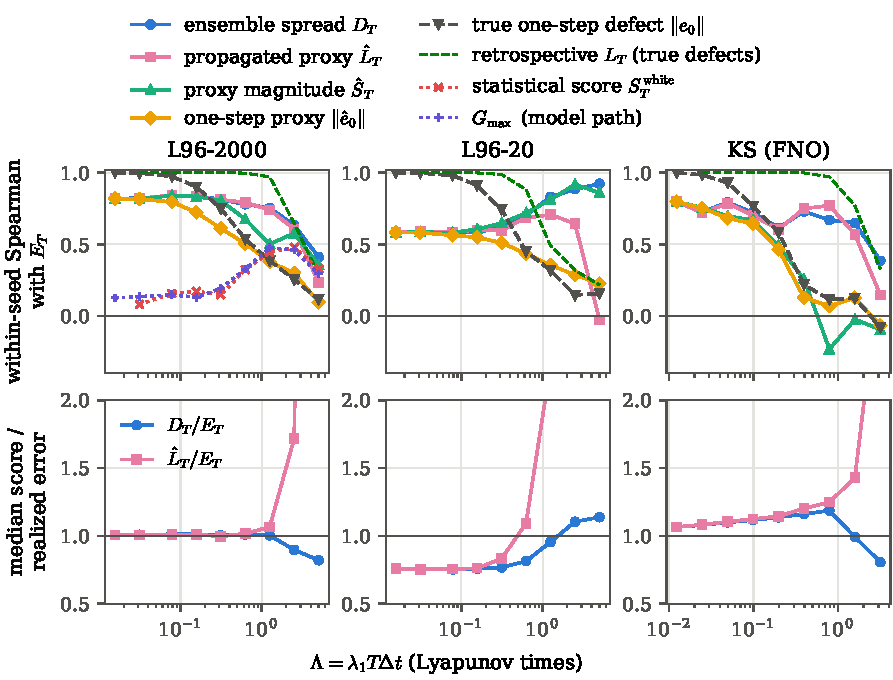
\includegraphics[width=\textwidth]{figures/fig_ensemble.pdf}
\caption{Reference-free error estimates. Top: within-seed Spearman correlation with $E_T$ of the ensemble spread, of the propagated, cumulative and one-step defect proxies, and, for comparison, of the true one-step defect, of the retrospective first-order reconstruction $L_T$ and (L96-2000) of two scores built from the defect statistics only. Bottom: median ratio between the spread or the propagated proxy and the realized error.}
\label{fig:ensemble}
\end{figure}

Two limitations are apparent. First, the under-trained L96-20 surrogates make similar errors, so that the proxy has a cosine of only $0.63$ with the true defect and $77\%$ of its norm, and the spread underestimates the error by $19$ to $25\%$ up to $0.63$ Lyapunov times. Its ranking is nevertheless good at long horizons ($0.83$ at $1.25$ Lyapunov times), where the error of these surrogates is dominated by the drift of their free rollouts. Second, beyond the validity of the first-order description, $\hat L_T$ overestimates the error strongly, whereas the nonlinear spread $D_T$ saturates with the forecasts and remains informative (correlations of $0.63$ for L96 at $2.5$ and of $0.65$ for KS at $1.58$ Lyapunov times).

\subsection{Multistep fine-tuning}
\label{sec:res_intervention}

Figure~\ref{fig:intervention} and Table~\ref{tab:intervention} summarize the fine-tuning study. For the L96-20 surrogates, the rollout arm reduces the test error of all five seeds at every horizon from $T=4$ on, and the median paired reduction grows from $1.2\%$ at $T=16$ to $11.5\%$ at $T=128$ over 312 non-overlapping windows of a common held-out trajectory. The factorization shows how this reduction is obtained. At $1.25$ Lyapunov times ($T=80$), the median over seeds of the mean change of the log-error is $-0.074$, of which $-0.054$ comes from the worst-case tail gain, $-0.010$ from the cancellation and $-0.012$ from the nonlinear factor, whereas the defect magnitude and the efficiency change by less than $0.2\%$. The multistep objective therefore acts on the learned tangent dynamics rather than on the defects. Along the reference trajectory, the median of $\log\sigma_1[\Phir(T,0)]$ of the L96-20 surrogates is already lower than that of the exact tangent map, by $0.26$ at $T=80$; the one-step arm leaves this deficit almost unchanged ($0.28$) and the rollout arm increases it to $0.36$, while the L96-2000 surrogates reproduce the reference value within $0.01$. The rollout arm also reduces the amplitude drift of the free rollout, with a median ratio between forecast and reference amplitudes of $1.19$ at $T=64$, against $1.28$ for the one-step arm. For these under-trained surrogates, the multistep objective thus lowers the error by damping the learned dynamics, at the cost of a larger departure from the reference tangent dynamics.

\begin{figure}[!tp]
\centering
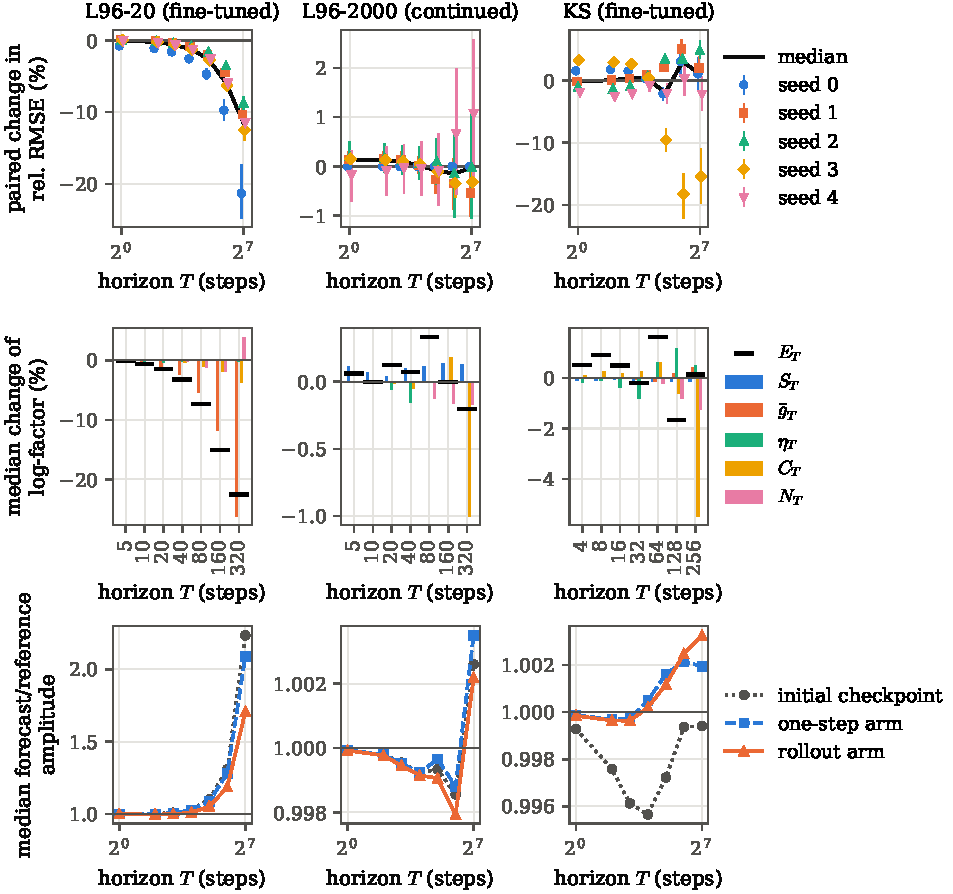
\includegraphics[width=\textwidth]{figures/fig_intervention.pdf}
\caption{Multistep fine-tuning. Top: paired change of the test relative RMSE (rollout arm against one-step arm) for every seed, with window-bootstrap 95\% intervals, and median over seeds. Middle: median over seeds of the mean change of the log-error and of its five factors on the diagnostic windows. Bottom: median ratio between the amplitudes of the forecast and of the reference state.}
\label{fig:intervention}
\end{figure}

\begin{table}[t]
\centering
\small
\caption{Median over five seeds of the paired change of the test relative RMSE (\%) between the rollout and the one-step arms, with the number of seeds improved by the rollout arm. Seed-level values and intervals are given in Appendix~\ref{app:tables}.}
\label{tab:intervention}
\begin{tabular}{lrrrr}
\toprule
Case & $T=16$ & $T=32$ & $T=64$ & $T=128$\\
\midrule
L96-20 & $-1.22$ (5/5) & $-2.60$ (5/5) & $-5.92$ (5/5) & $-11.46$ (5/5)\\
L96-2000 & $+0.02$ (1/5) & $-0.08$ (3/5) & $-0.15$ (3/5) & $-0.03$ (3/5)\\
KS & $+0.44$ (1/5) & $-2.04$ (3/5) & $+3.07$ (1/5) & $+1.09$ (2/5)\\
\bottomrule
\end{tabular}

\end{table}

The converged surrogates do not benefit from the multistep objective. For L96-2000, the paired changes are below $0.2\%$ in median at all horizons, with one to three of five seeds improved, and the window-bootstrap intervals of most seeds include zero. On the diagnostic windows, the mean change of the log-error and of every factor is below $0.4\%$ up to $2.5$ Lyapunov times. For the FNOs, the effects change sign between seeds and horizons. One seed improves by $9.5$ to $18.2\%$ between $T=32$ and $128$, two seeds become worse by $2$ to $5\%$, and the remaining two change sign between horizons (Appendix~\ref{app:tables}). The factors that change also differ between seeds, and neither the magnitude nor the worst-case gain changes systematically. Under the tested budgets, the benefit of the multistep objective in Lorenz--96 is therefore an effect of under-training, obtained by damping a learned map whose free rollouts leave the attractor, and it disappears when the surrogate reproduces the tangent dynamics of the reference system.
